\chapter{Proposed Approach}
\label{ch:prop}

The contributions of this project can be seen as two main categories of research work. The first set was accomplished in the beginning phase of this project: behavioral and explicit error propagation through the implemenation of the Safety Annex for AADL. The remaining pieces of this research provide the bulk of the contribution and consist of the compositional generation of minimal cut sets through the transformation of inductive validity cores and using the fault tree generated by this transformation to compute the probability of a safety property violation. 

\section{Behavioral and Explicit Error Propagation}
The usage of the terms error, failure, and fault are defined in ARP4754A and are described here for ease of understanding~\cite{SAE:ARP4754A}. An \textit{error} is a mistake made in implementation, design, or requirements. A \textit{fault} is the manifestation of an error and a \textit{failure} is an event that occurs when the delivered service of a system deviates from correct behavior. If a fault is activated under the right circumstances, that fault can lead to a failure. The term \textit{error propagation} is used to refer to the propagation of the corrupted state caused by an active fault. 

The Safety Annex is used to add possible faulty behaviors to a component model. Within the AADL component instance model, an annex is added which contain the fault definitions for the given component. The flexibility of the fault definitions allows the user to define numerous types of fault \textit{nodes} by utilizing the AGREE node syntax. Examples of such faults include valves being stuck open or closed, output of a software component being nondeterministic, or power being cut off.  

When a fault is activated by its specified triggering conditions, it modifies the output of the component. This faulty behavior may violate the contracts of other components in the system, including assumptions of downstream components. The impact of a fault is computed by the AGREE model checker when the safety analysis is run on the fault model; the error propagation is not explicitly defined as in some closely related tools~\cite{EMV2,compass30toolset}. 

On the other hand, failures in hardware (HW) components can trigger behavioral faults in the system components that depend on them. This makes it beneficial to allow for explicit error propagation and the definition of dependencies in the fault model. For example, a CPU failure may trigger faulty behavior in the threads bound to that CPU. In addition, a failure in one HW component may trigger failure in other HW components located nearby, such as overheating, fire, or explosion
in the containment location. The Safety Annex provides the capability to explicitly model the impact of hardware failures on other faults, behavioral or non behavioral. 

Users specify dependencies between the HW component faults and faults that are defined in other components, either HW or SW. The hardware fault then acts as a trigger for dependent faults. This allows a simple propagation from the faulty HW component to the SW components that rely on it, affecting the behavior on the outputs of the affected SW components. Within the implementation, this corresponds to a statement linking the active fault to all dependent faults. Thus, if the triggering fault is active, so are all dependencies.

\subsection{Implementation}
The Safety Annex is written in Java as a plug-in for the OSATE AADL toolset, which is built on Eclipse.  It is not designed as a stand-alone extension of the language, but works with behavioral contracts specified using the AGREE AADL annex~\cite{NFM2012:CoGaMiWhLaLu}. 
The architecture of the Safety Annex is shown in Figure~\ref{fig:plugin-arch}.

\begin{figure}[h!]
	\begin{center}
		%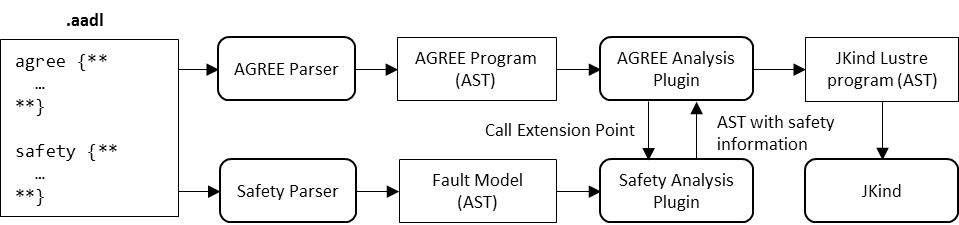
\includegraphics[trim=0 400 430 0,clip,width=0.85\textwidth]{images/arch.png}
		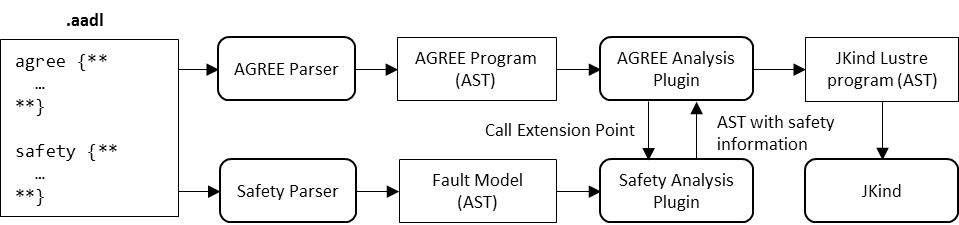
\includegraphics[width=\textwidth]{images/arch.png}
	\end{center}
	%\vspace{-0.1in}
	\caption{Safety Annex Plug-in Architecture}
	\label{fig:plugin-arch}
	%\vspace{-0.1in}
\end{figure}

AGREE contracts are used to define the nominal behaviors of system components as {\em guarantees} that hold when {\em assumptions} about the values the component's environment are met. When an AADL model is annotated with AGREE contracts and the fault model is created using the Safety Annex, the model is transformed through AGREE into a Lustre model~\cite{Halbwachs91:IEEE} containing the behavioral extensions defined in the AGREE contracts for each system component. 

When performing fault analysis, the Safety Annex extends the AGREE contracts to allow faults to modify the behavior of component inputs and outputs. An example of a portion of an initial AGREE node and its extended contract is shown in Figure~\ref{fig:lustre}. The left column of the figure shows the nominal Lustre pump definition is shown with an AGREE contract on the output; and the right column shows the additional local variables for the fault (boxes 1 and 2), the assertion binding the fault value to the nominal value (boxes 3 and 4), and the fault node definition (box 5). Once augmented with fault information, the AGREE model (translated into the Lustre dataflow language~\cite{Halbwachs91:IEEE}) follows the standard translation path to the model checker JKind~\cite{2017arXiv171201222G}, an infinite-state model checker for safety properties. 

\begin{figure}[h!]
	\hspace*{-2cm}
	%\vspace{-0.1in} 
	\begin{center}
		%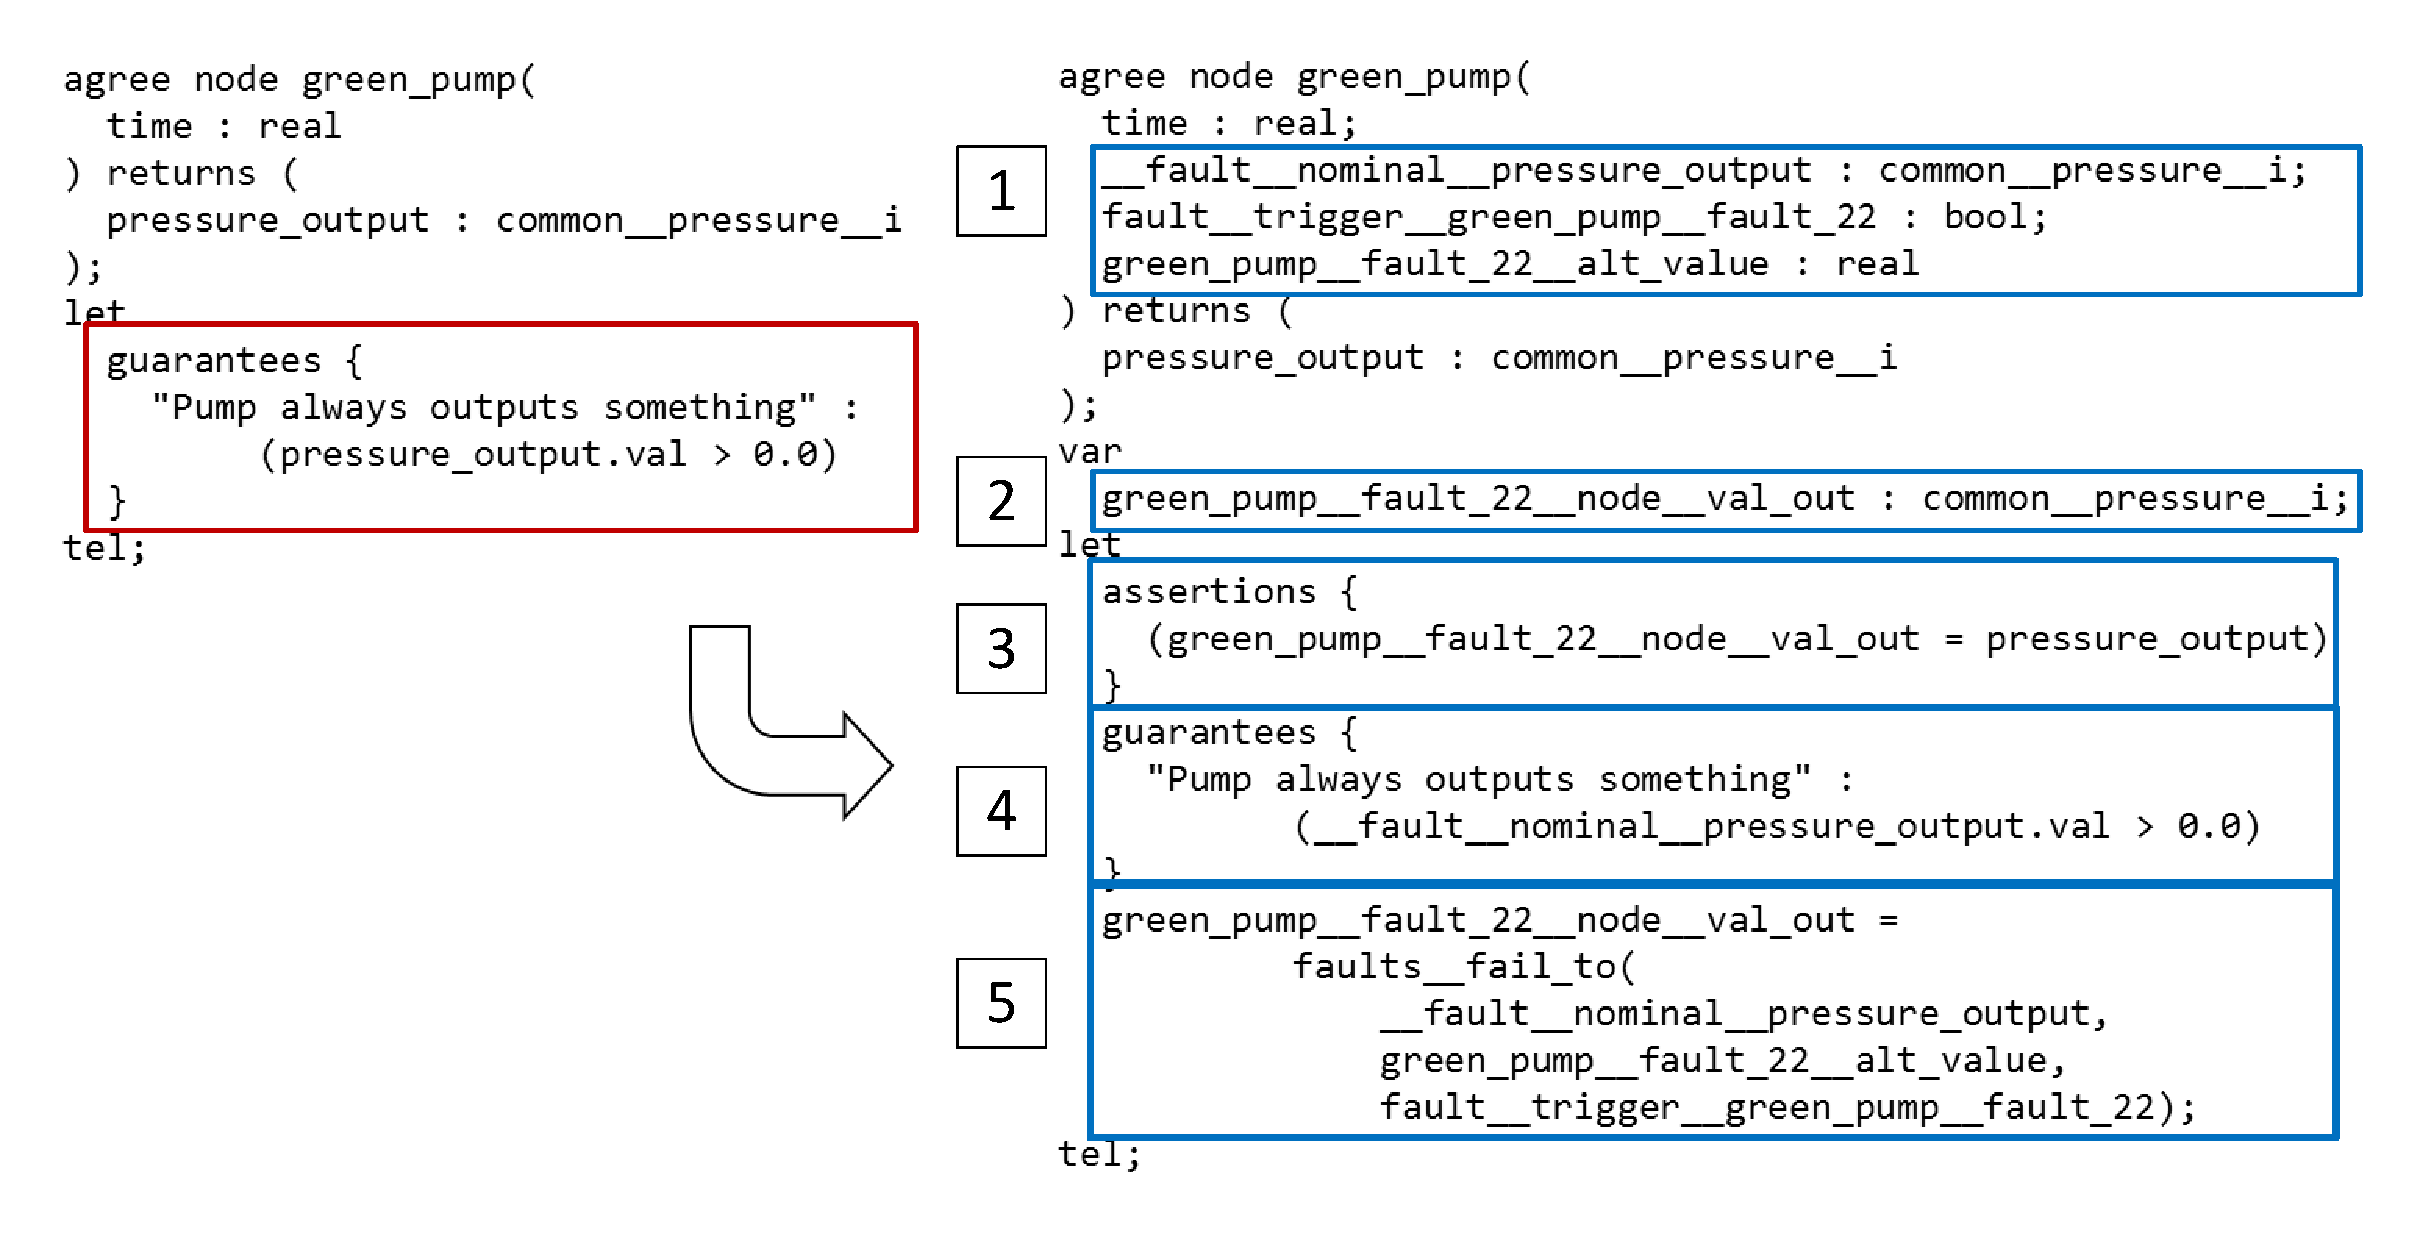
\includegraphics[trim=0 690 -10 70,clip,width=1.5\dimexpr\textwidth-2cm\relax]{images/lustre.pdf}
		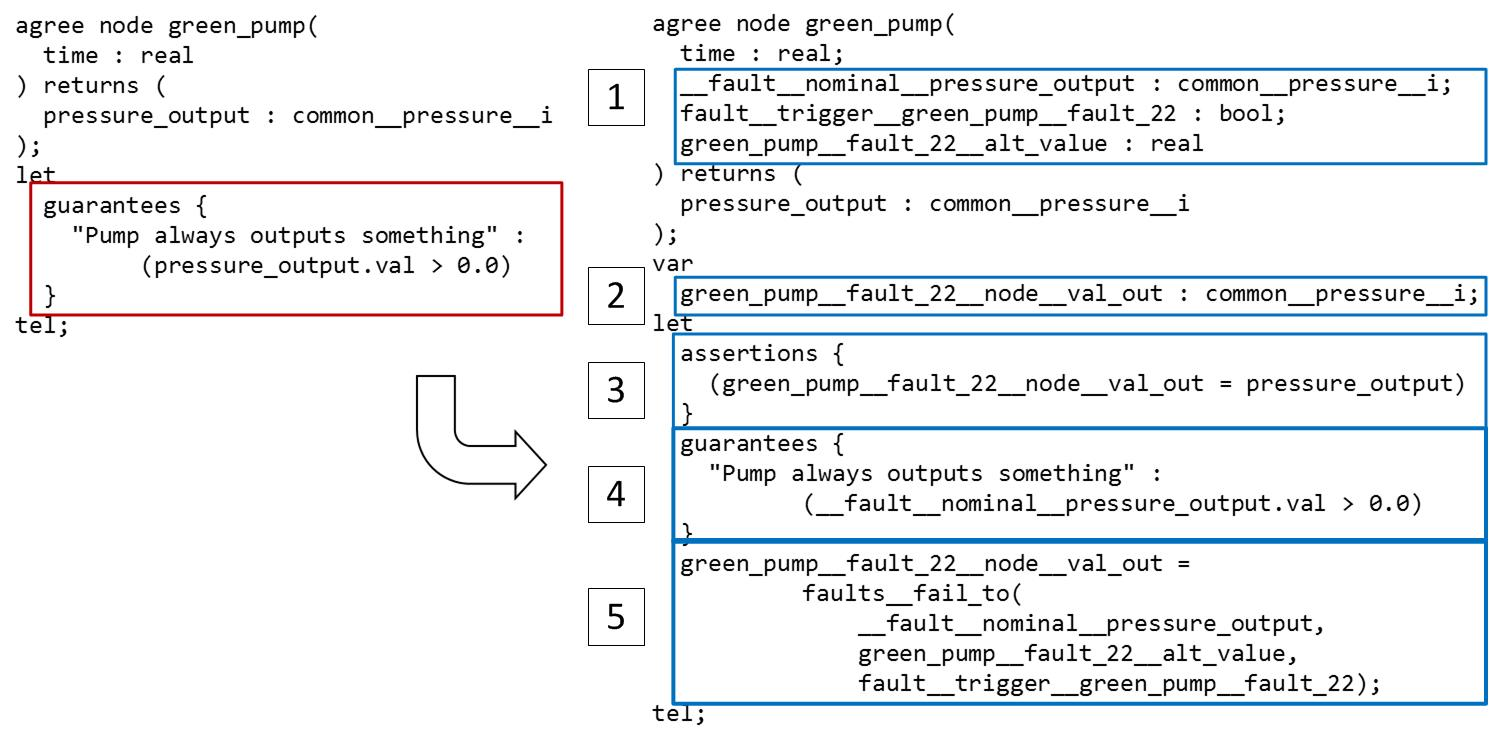
\includegraphics[scale=0.3]{images/lustre.jpg}
		%\caption{Nominal AGREE node and its extension with faults}
		\caption{Nominal AGREE Node and Extension with Faults}
		\label{fig:lustre}
	\end{center}
	%\vspace{-0.1in}
\end{figure}


\section{Generation of Minimal Cut Sets from MIVCs}
As was previously explained, the MIVCs are MUSs of a constraint system. The MCSs (Minimal Correction Sets) can be obtained through the use of a hitting set algorithm. The MCSs can be seen as a correction of the infeasability of the constraint system. Recall that the constraint system consists ofsubcomponent contracts, or guarantees, constrained to true, fault activation literals constrained to false, and the \textit{negation} of the safety property. Under the assumption that the nominal system is satisfiable (when no faults are active, the property proves), it is no surprise that the constraint system framed this way is unsatisfiable. 

The MCS provides a correction to that infeasability; thus, if the constraints on the elements in the MCS are removed from the constraint system, that system is now satisfiable. If the guarantees are no longer constrained to true and the fault activation literals are not constrained to false, the negation of the safety property \textit{with these unconstrained elements} is now satisfied. These correspond to the minimal set of faults and violated guarantees that cause violation of the safety property. 

The basic idea of the proposed algorithm is to collect all MIVCs, transform them into MCSs (Minimal Correction Sets) by the use of a hitting set algorithm, and then transform the MCSs into MinCutSets. It is a requirement of the minimal hitting set algorithm that \textit{all} MUSs are used to find the MCSs~\cite{liffiton2016fast,gainer2017minimal,murakami2013efficient}. Thus, once all MIVCs have been found and the minimal hitting set algorithm has completed, the MinCutSet generation algorithm can begin. 

%Initially, we begin with a list of MCSs for each layer. As mentioned previously, at the leaf layer this set only contains constrained faults, but at intermediate layers it is possible for the MCSs to contain a mixture of both constrained inactive faults and valid contracts. When this is the case, a replacement must be made between the contracts and the faults in the model that can cause their violation. Once this replacement begins, this set is no longer an MCS nor is it yet a MinCutSet. We call this set $I$ for \textit{Intermediate Set} in the following algorithm. 

%Initially, we begin
The MinCutSet generation algorithm begins with a list of $MCSs$ specific to a top level property. Since MIVCs can contain fault activation literals constrained to \textit{false} and and subcomponent contracts constrained to \textit{true}, the $MCSs$ may also contain this mixture. Minimal cut sets only contain faults, and thus the MCSs require additional processing in order to be considered MinCutSets.

Since we assume that the nominal model proves, if any contracts are violated this is due to an active fault in the system. Each contract will then have it's own minimal cut set. Given that MIVCs are collected compositionally, each subcomponent contract has a set of minimal model elements required for its proof. These correspond (on the lowest level) to fault activation literals constrained to false. Once these are collected for the contracts in question, a replacement can be made in the MCS. The violated contract is replaced by the active fault literals that caused its violation. In the end, the MCS is transformed into a MinCutSet.

%We remove all constraints from each $MCS$ and call the resulting sets $I$, for \textit{Intermediate} set. Replacement of subcomponent contracts with their respective minimal cut sets can then proceed. For each of those contracts in $I$, we check to see if we have previously obtained a $MinCutSet$ for that contract. If so, replacement is performed. If not, we recursively call this algorithm to obtain the list of all %$MCSs$ 
%MinCutSets associated with this subcomponent contract. At a certain point, there will be no more contracts in the set $I$ in which case we have a minimal cut set for the current property. When this set is obtained, we store it in a lookup table keyed by the given property that this $I$ is associated with. 

%Initially, we begin with a list of MCSs for each layers contracts. At the leaf layer, the MCSs only contain constrained to inactive faults, and we remove the constraints to obtain MinCutSet for each component contract at the leaf layer. At the intermediate layers, the MCSs can contain a mixture of constrained inactive faults and valid component contracts. We first remove the constraints on them to obtain an \textit{Intermediate Set}, $I$, that contains active faults and invalid subcomponent contracts, and replace each invalid subcomponent contract with the MinCutSet obtained for that contract from the layer below. We call this intermediate set $I$ in the following algorithm and $List(I)$ is the set of all $MCSs$ for a component contract at the start of the algorithm and all intermediate sets once replacement begins. At the end of the algorithm the minimal cut sets for the top level property are generated.

%Notes regarding the following algorithm: at the onset, the current property $P$ is a top level property. Each of the properties has a list of associated $MCSs$. When the algorithm states that constraints on these elements are removed, more specifically the fault activation literals in $MCS$ are constrained to \textit{true} and the component contracts are constrained to \textit{false}. $List(I)$ is the collection of all $MCSs$ with all constraints removed. Assuming All-MIVCs have been found and the minimal hitting set algorithm has terminated, giving us a list of $MCSs$ for each property in the system. 

The formal proofs showing that this transformation is possible will be provided and the algorithms will be implemented in the Safety Annex.  


\section{Probabilistic Computations over the Fault Tree}














\begin{comment}
\section{Fault Tree Analysis} 
The use of fault trees are common in many safety assessment processes and the ability to generate the cut sets needed for the construction of the fault tree is a useful part of any safety analysis tool. The fault tree is a safety artifact commonly referenced in requirement protocol documents such as ARP4761, ARP4754, and AIR6110~\cite{SAE:ARP4761,SAE:ARP4754A,AIR6110}.

A Fault Tree (FT) is a directed acyclic graph whose leaves model component failures and whose gates model failure propagation~\cite{0f356f05e72f43018211b36f97c8854a}. The system failure under examination is the root of the tree and is called the Top Level Event (TLE). The node types in a fault tree are \textit{events} and \textit{gates}. An event is an occurrence within the system, typically the failure of a subsystem down to an individual component. Events can be grouped into Basic Events (BEs), which occur independently, and \textit{intermediate events} which occur dependently and are caused by one or more other events~\cite{historyFTA}.  These events model the failure of the system (or subsystem) under consideration. The gates represent how failures propagate through the system and how failures in subsystems can cause system wide failures. The two main logic symbols used are the Boolean logic AND-gates and OR-gates. An AND-gate is used when the undesired top level event can only occur when all the lower conditions are true. The OR-gate is used when the undesired event can occur if any one or more of the next lower conditions is true. This is not a comprehensive list of gate types, but we focus our attention on these two common gate types. 
\begin{figure}[h]
\begin{center}
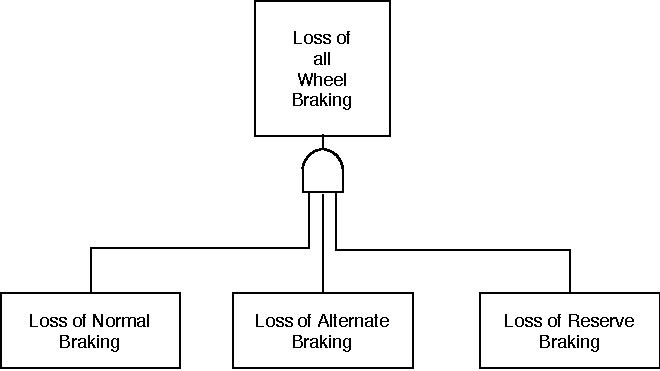
\includegraphics[width=8cm]{images/introFT2.pdf}
\caption{A simple fault tree} \label{fig:introFT}
\end{center}
\end{figure}

Figure~\ref{fig:introFT} shows a simple example of a fault tree based on SAE ARP4761~\cite{SAE:ARP4761}. In this example, the top level event corresponds to an aircraft losing all wheel braking. In order for this event to occur, all of the basic events must occur. This is seen through the use of the AND gate below the top level event. The gates in the fault tree describe how failures propagate through the system. Each gate has one output and one or more inputs. In Figure~\ref{fig:introFT}, the AND gate has three inputs and one output. The leaves of the tree represent the basic events of the system. %and 
In the case of this fault tree, these three events are also the Minimal Cut Sets (MinCutSets) for this top level event. A MinCutSet is the minimal set of basic events that must occur together in order to cause the TLE to occur. Generating and analyzing these MinCutSets is important to FTA and has been an active area of interest in the research community since fault trees were first described in Bell Labs in 1961~\cite{historyFTA,0f356f05e72f43018211b36f97c8854a}. 

There are two main types of fault tree analysis that we differentiate here as \textit{qualitative} analysis and \textit{quantitative} analysis. In qualitative analysis, the structure of the fault tree is considered and the MinCutSets are a way to indicate which combinations of component failures will cause the system to fail. On the other hand, in quantitative analysis the probability of the TLE is calculated given the probability of occurrence of the basic events. By being able to generate MinCutSets
based on both cardinality and probability, this allows for either form of FTA to be created. 


\end{comment}